\begin{Minutes}{Bayesian Multi-modal MR discussion}
%%\subtitle{}
%%\moderation{}
%%\minutetaker{}
\participant{David Knowles, Stephen Malina, Brielin Brown}
%%\missingExcused{}
%%\missingNoExcuse{}
\minutesdate{February 26, 2020}
%%\starttime{}
%%\endtime{}
%%\cc{}
\maketitle
\topic{Overview}
We discussed a few topics:
\begin{enumerate}
    \item Mimicking the zero modal pleiotropy MR method using a mixture of Gaussians model
    \item Next steps for Deep MR
\end{enumerate}

I've included my pictures of the whiteboard from our discussion at the end of
these notes.

\topic{Bayesian MR}
\subtopic{Bi-directional MR issue}
Brielin is interested in the `Bayesian' approach to bi-directional MR because
he's discovered an issue with using significance as a proxy for picking instruments
in bi-directional MR. Selecting instruments based on significance leads to problems
when we have different sample sizes for different pairings of the instrument and
phenotypes we're looking at. E.g., say \( I \) is an instrument for \( A \) which
actually causes \( B \), but I only have a few samples of \( i, a \) and many
samples of \( i, b \). As a result, it's possible that I'll guess that
\( I \) is an instrument for \( B \). If I do this, then my Wald estimator
for \( B \rightarrow A \), \( \hat{\beta}_{B \rightarrow A} \) will be
\( \frac{1}{\beta} \) where \( \beta \) is the true causal effect of
\( A \) on \( B \).

\subtopic{Mixture model}
(This describes the model depicted in~\ref{fig:2}.)
We want to parameterize a (eventually, mixture of) Gaussian by a radius (\( \rho \))
and angle parameter (\( \theta \)) to approximate the non-Bayesian zero modal
pleiotropy model. David described a hierarchical model as an approach
for doing so. The model assumes that we have computed a set of effect sizes,
\( (\hat{\beta}_{iA}, \hat{\beta}_{iB}), \dots \) and standard errors
\( \hat{\sigma}_{iA}, \hat{\sigma}_{iB} \) where \( A, B \) correspond to the
\( Z \rightarrow X \) and \( Z \rightarrow Y \) relationships respectively.

To describe the model, we start with the assumption that effect sizes
for each variant (indexed by \( i \)) are jointly normally distributed,
\begin{align*}
    \begin{bmatrix} \hat{\beta}_{iA} \\ \hat{\beta}_{iB} \end{bmatrix} \mid \theta, \rho \sim \text{Normal}\left(\rho \begin{bmatrix} \cos \theta \\ \sin \theta \end{bmatrix}, \text{diag}\left(\begin{bmatrix} \sigma_{iA} & \sigma_{iB} \end{bmatrix}^\top\right)\right).
\end{align*}
Since \( \rho \) is a nuisance parameter in this model, we can integrate it out. Letting \[ \mathbf{t} = \begin{bmatrix}
    \cos \theta_i \\
    \sin \theta_i
\end{bmatrix}, 
\]
we have
\begin{align*}
    \begin{bmatrix} \hat{\beta}_{iA} \\ \hat{\beta}_{iB} \end{bmatrix} \mid \theta \sim \text{Normal}\left(0, \mathbf{t}\mathbf{t}^\top + \text{diag}\left(\begin{bmatrix} \sigma_{iA} & \sigma_{iB} \end{bmatrix}^\top\right)\right).
\end{align*}

Next we need to put priors on our parameters. For our angles, \( \theta_1, \dots, \theta_n \), we have
\[ \theta \sim \text{VM}(\mu, \kappa) \]
where \( \text{VM} \) denotes the \hyperlink{https://en.wikipedia.org/wiki/Von_Mises_distribution}{Von Mises distribution} over the circle.

Then, our inferred distribution over \( \theta \)s should reflect SNP-specific causal effects and
our distribution over \( \mu \) should reflect the 'overall' causal effect.

This covers the basics of the unimodal version of the model. Obviously, there's still a bunch of details on how to fit this thing, but
I'll leave those for when I'm actually doing the work.

The other thing I wanted to note is what the \( c_i \) terms in
figure~\ref{fig:2} represent. The novel use-case for this model relates to
Brielin's stuff about bi-direcitonal MR I discussed above. Solving the
bi-directional MR problem requires dealing with a bi-modal distribution of
effect sizes, so the \( c_i \)s and the discrete distribution over them
reflect that.

\begin{figure}[htp]
    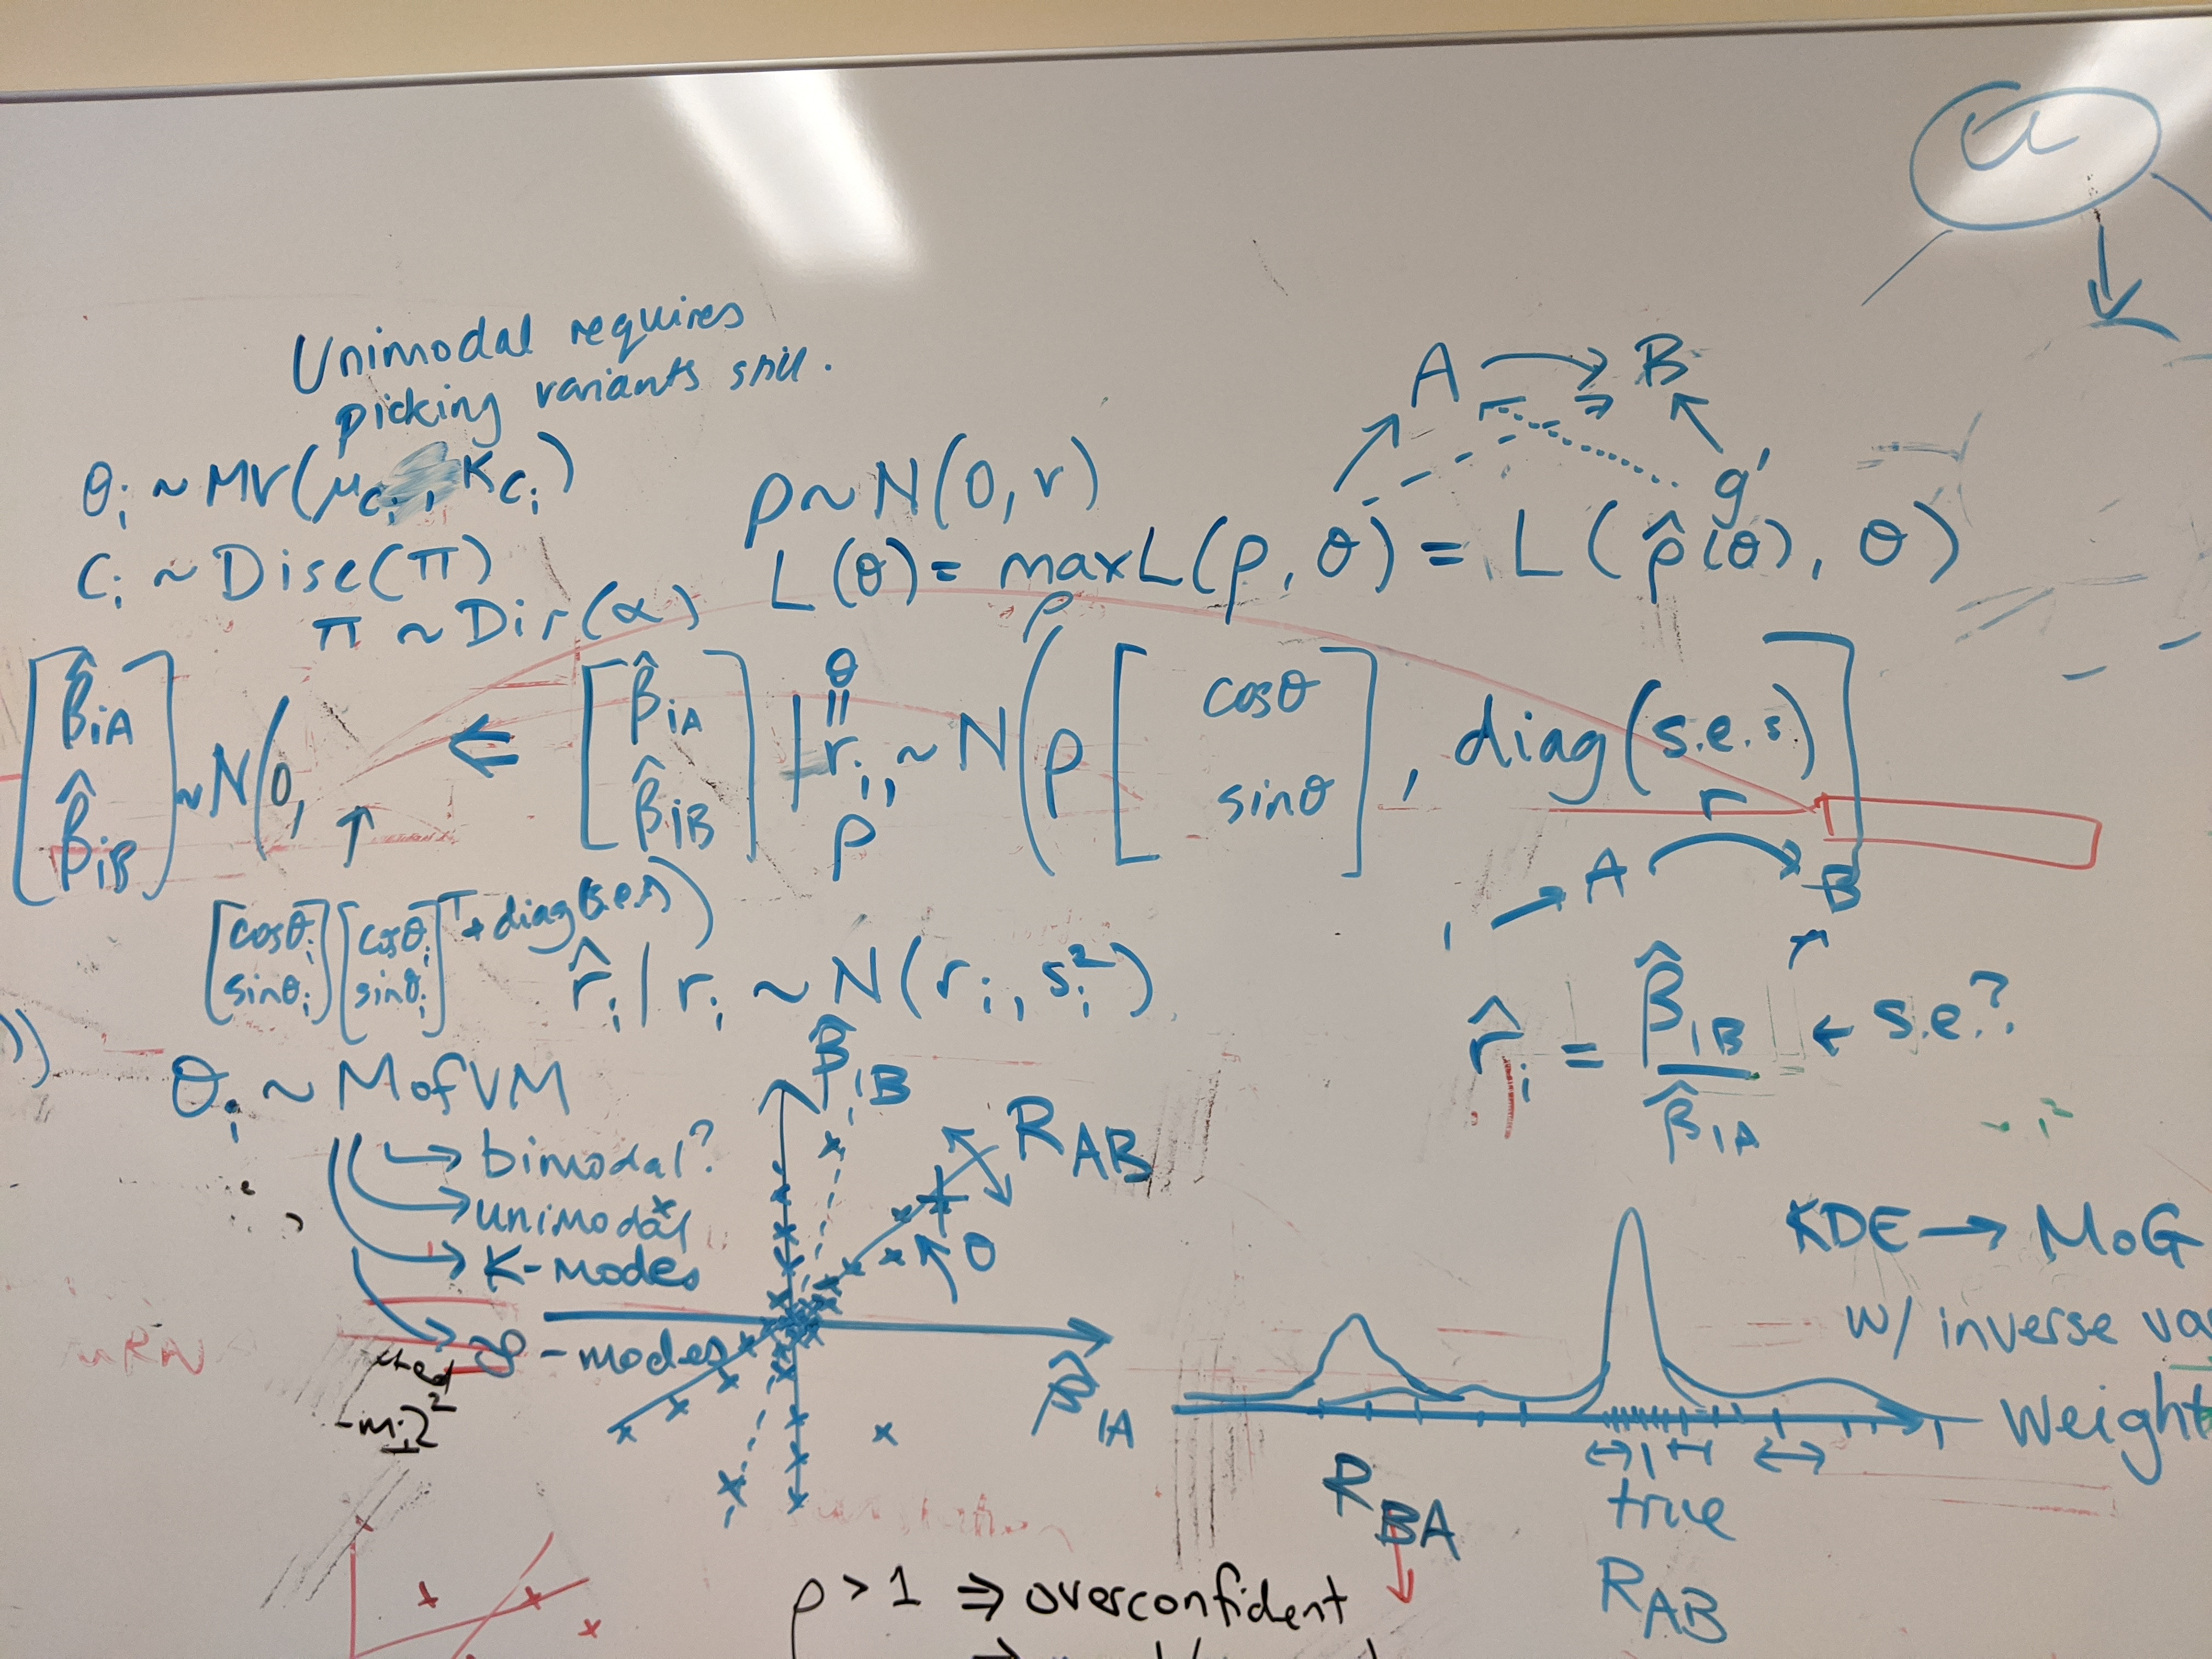
\includegraphics[width=.9\textwidth]{figures/whiteboard_20200226_2}
    \label{fig:2}
    \caption{Mixture of Gaussians model for unimodal MR.}
\end{figure}
\begin{figure}[h]
    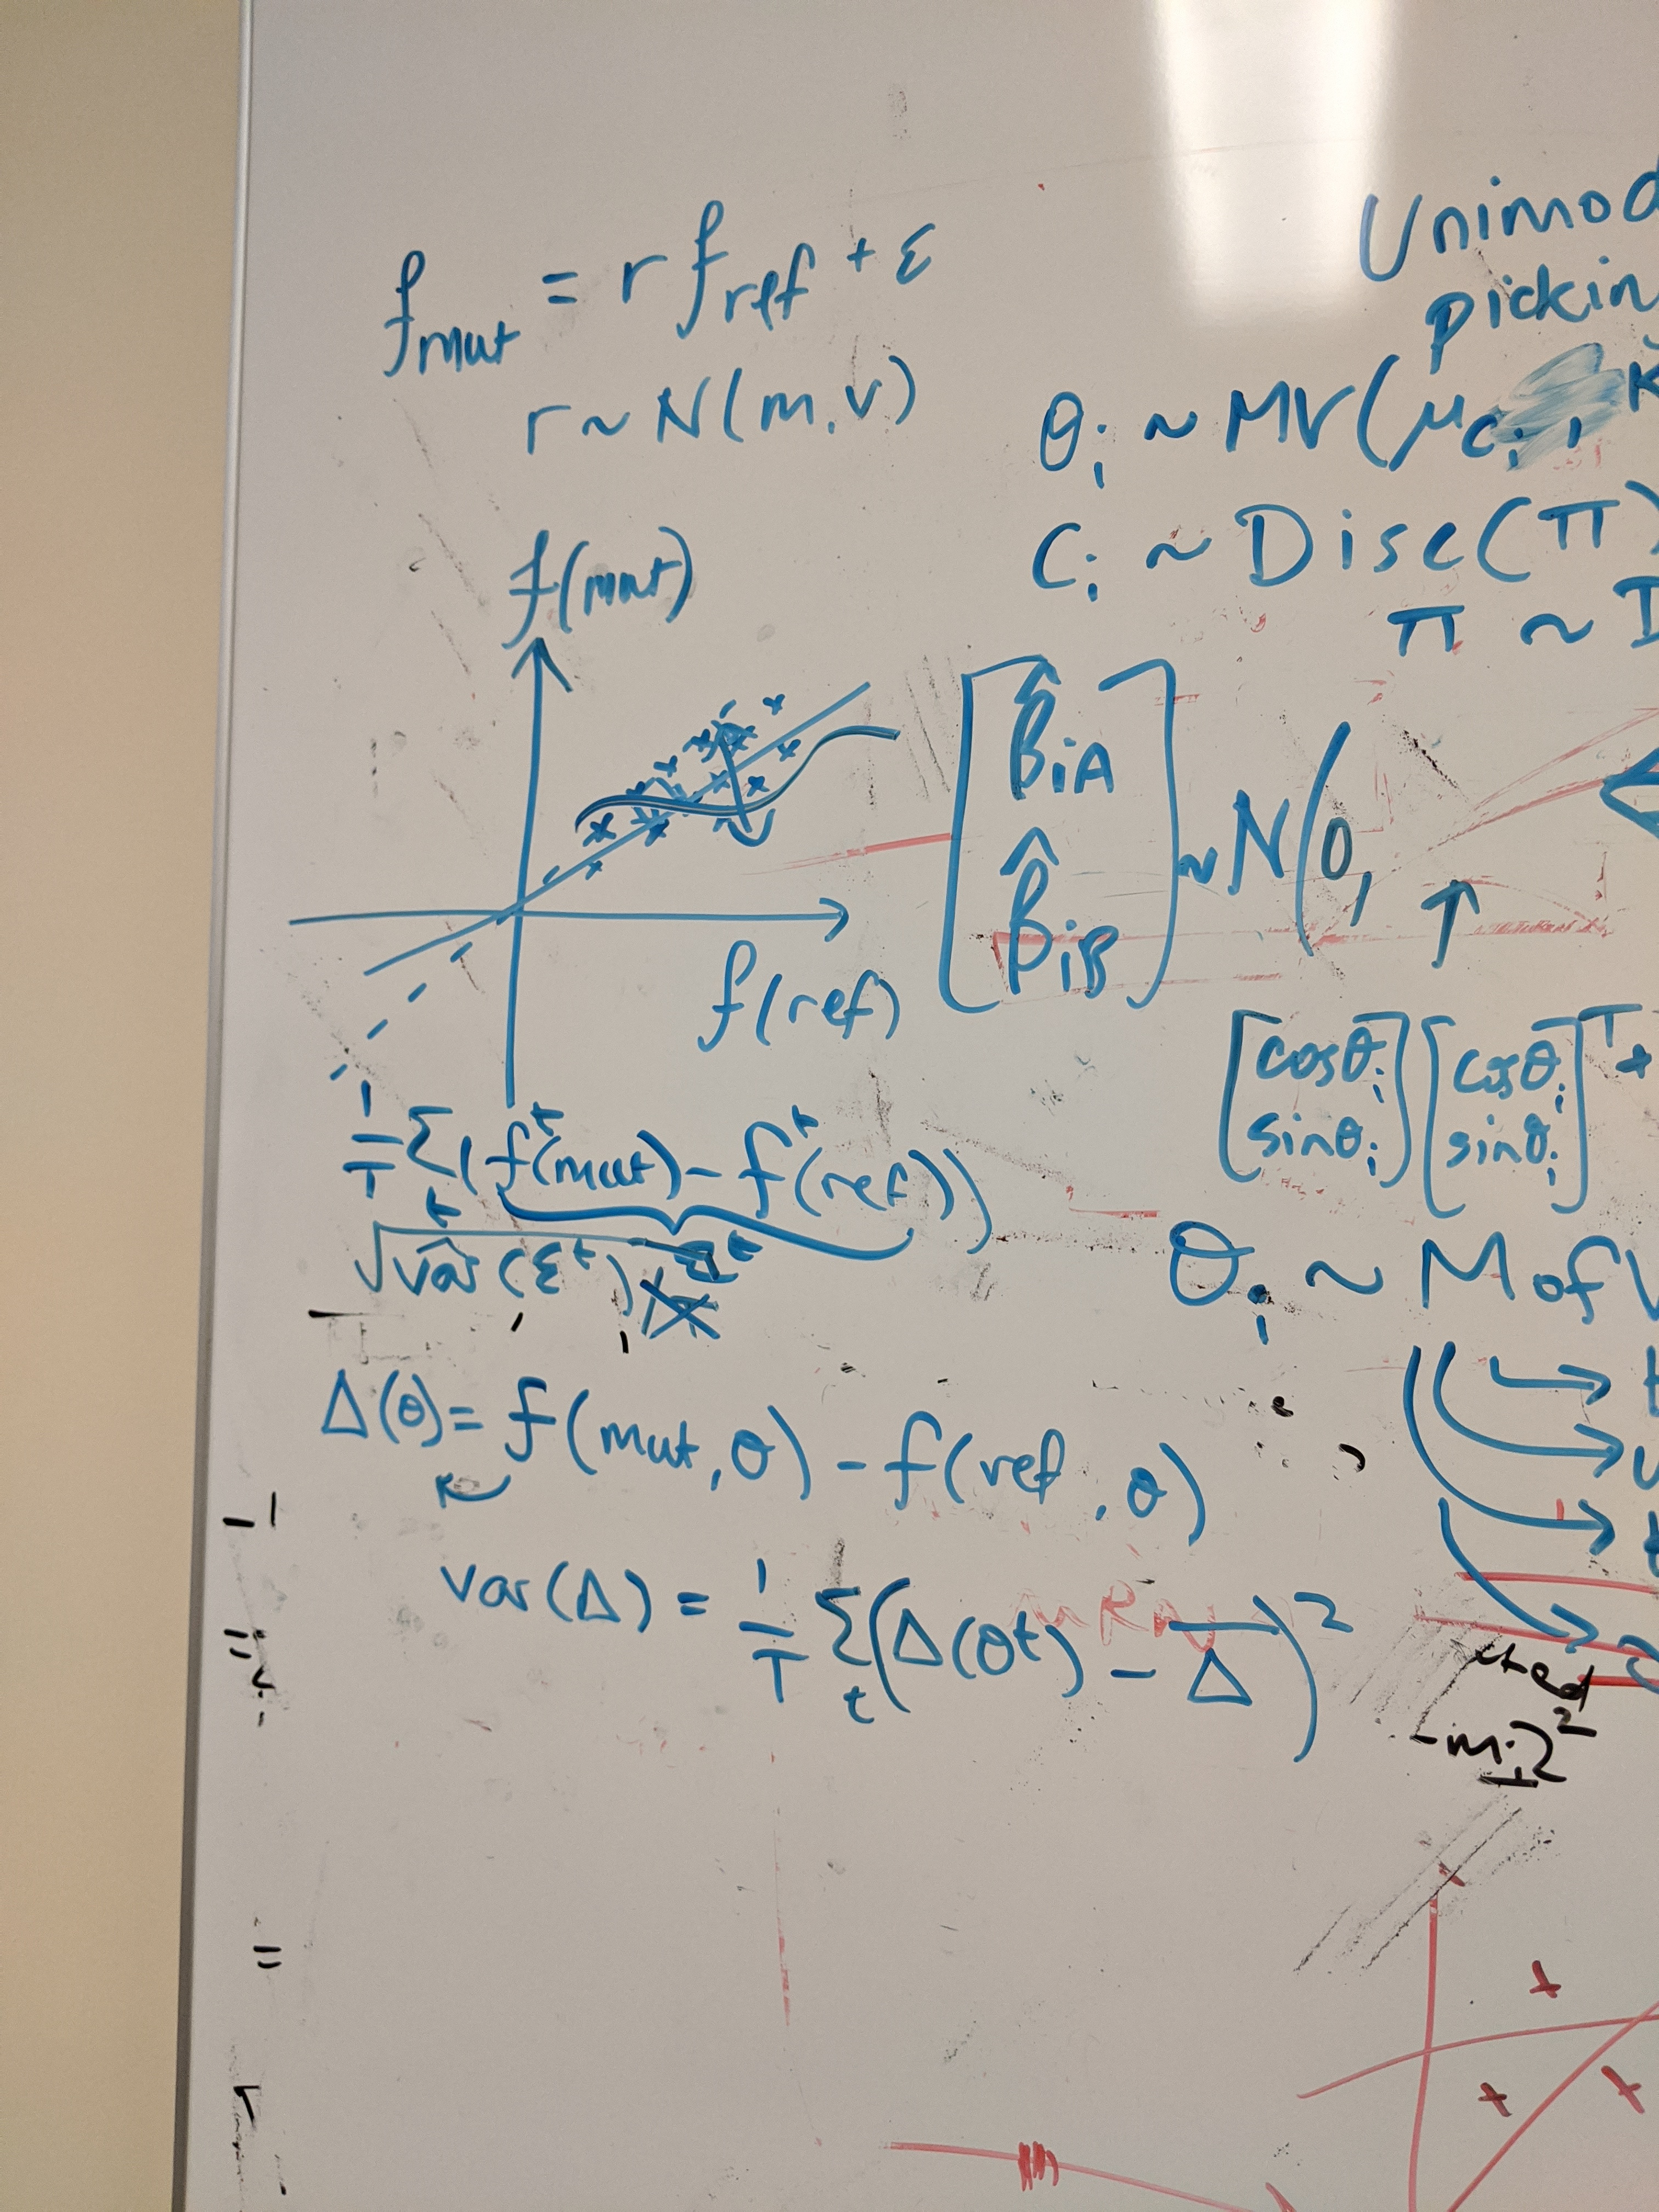
\includegraphics[width=.9\textwidth]{figures/whiteboard_20200226_3}
    \label{fig:2}
\end{figure}
\begin{figure}[h]
    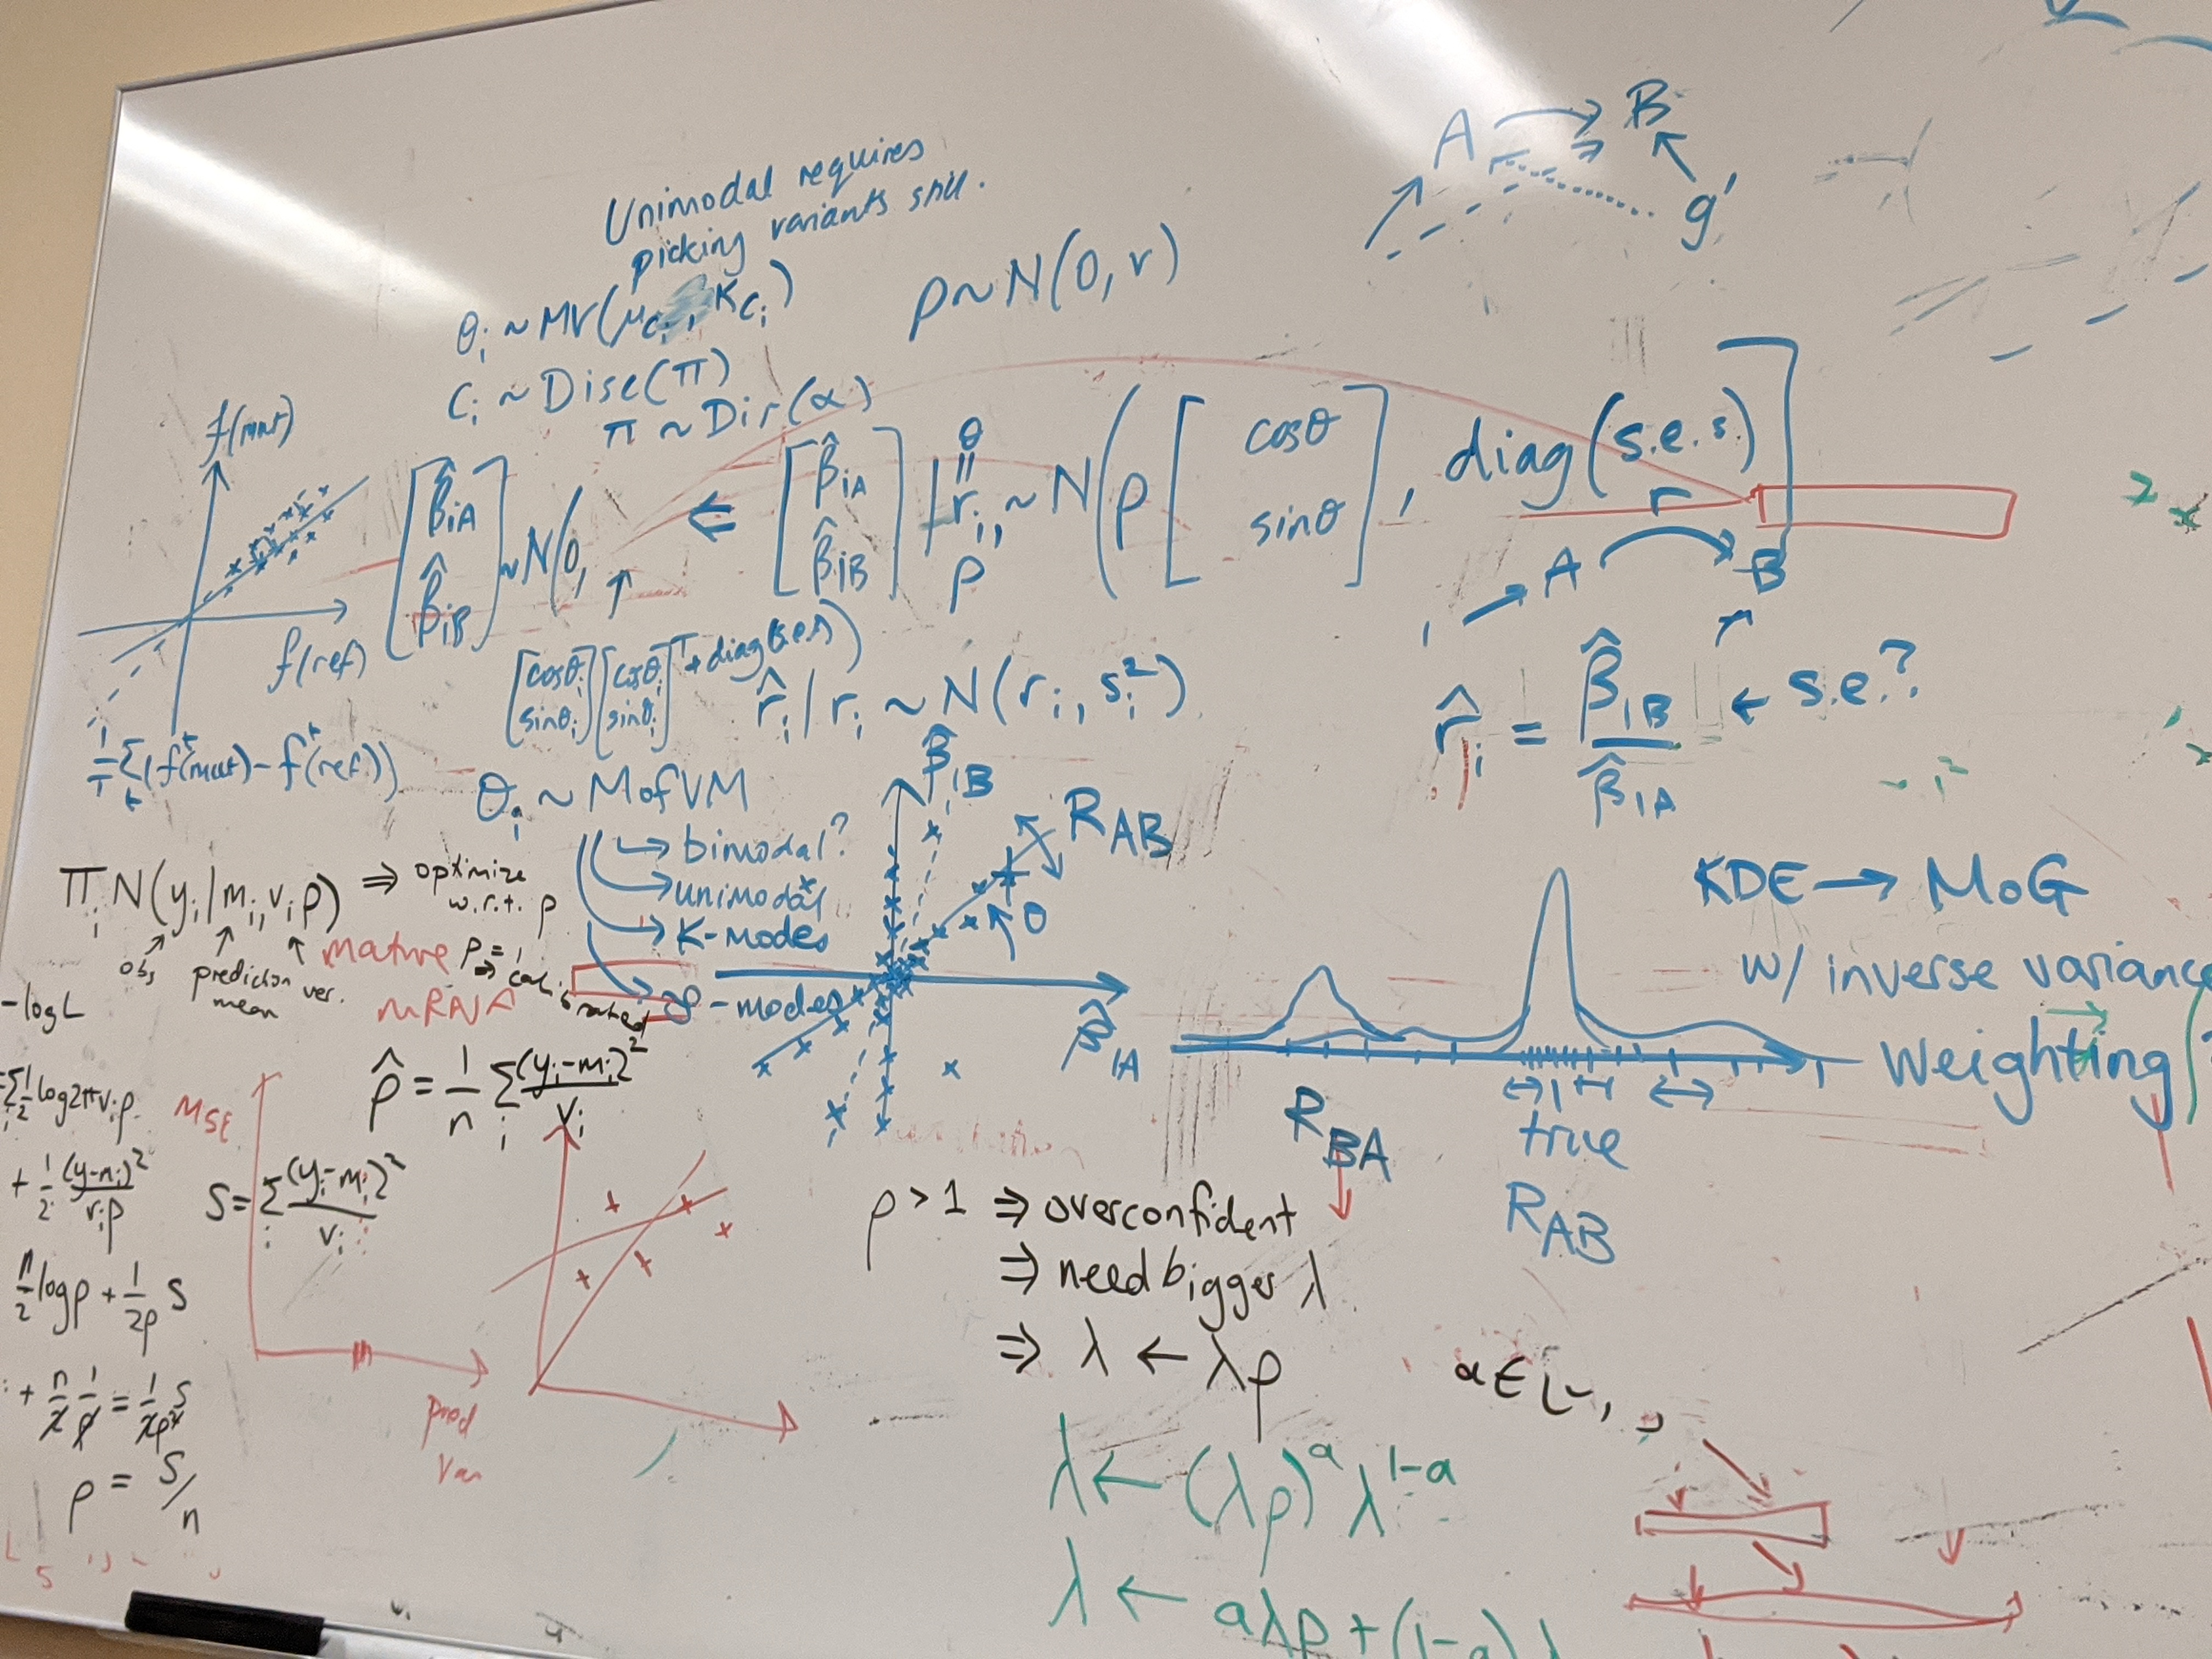
\includegraphics[width=.9\textwidth]{figures/whiteboard_20200226_1}
\end{figure}

\end{Minutes}
